\subsection{Knots and diagrams}

{\large\color{red}KTO CO ROBIŁ}

In mathematical terms, a knot is a particular embedding $S^1\hookrightarrow S^3$. A knot diagram is a {\color{blue}immersive projection} $D:S^1\twoheadrightarrow \R^2$ along a vector such that no three points of the knot lay on this vector \cite{likorish-diagram}.

$S^1$ is an orientable space thus we can choose an orientation for a knot being considered. Then a diagram $D$ is oriented if it is a projection of an oriented $S^1$.

Intuitively, two knots $K_1$ and $K_2$ are equivalent if we can deform one into the other without cutting it and only manipulating it with our hands \cite{murasagi-equivalence}. This translates to equivalence of diagrams, which is generated by a set of moves, called the \buff{Reidemeister moves}. In the case of a diagram without an orientation, three moves are sufficient. When an orientation is imposed on $D$, $4$ diagram moves generate the whole equivalence relation on diagrams \cite{ruchy_zorientowane}.

\subsection{Knot group}

Let $K$ be a knot and $D$ be its oriented diagram with $s$ segments and $x$ crossings. 
%The knot itself has the homotopy type of a circle and so its fundamental group is not interesting in itself. However, for a knot that is embedded in $S^3$ we can study the fun
\begin{definition}[knot group] 
  The fundamental group of a knot embedded in a three dimensional sphere $S^3$ is called a \buff{knot group}.
  $$\mathbf{\pi_1(K):=\pi_1(S^3-K)}.
  $$
\end{definition}
Although the knot itself has the same homotopy type as a circle, the knot group has usually an interesting yet difficult structure. The most known representation of the knot group is called \buff{the Wirtinger presentation}.

\begin{definition}[Wirtinger presentation]
  {\large\color{red}to do}
\end{definition}

An easily obtainable result, either by applying the Mayer-Vietoris sequence to $S^3=K\oplus S^3-K$ or noticing that every two generators are conjugate, is that the abelianization of the knot group is always $\Z$. This leads to an acyclic complex
\begin{center}
  \begin{tikzcd}
    0\arrow[r] & K \arrow[r] & G=\pi_1(K)\arrow[r, "ab"] & \Z=G^{ab} \arrow[r] & 0
  \end{tikzcd}
\end{center}

If $G$ is considered in its Wirtinger presentation, then $K$ does not have a finite set of generators. If $a_1$,..., $a_s$ where the generators of $G$ such that $(a_i)^{ab}=1$ for every $i$, then choosing new generators to be $x_i=a_ia_1^{-1}$ for $i=2,..., s$ implies that $K$ is generated by $a_1^{k}x_ia_1^{-k}$ for $i=2,...,s$ and $k\in\Z$.

\begin{definition}[metabelianization]
  Let $G$ be a knot group and let $K=\ker(ab:G\to \Z)$. Then we call $G^{mab}=G/[K, K]$ the \buff{metabelianization} of $G$. 
\end{definition}

{\color{blue}
The following exact sequence is exact
\begin{center}
  \begin{tikzcd}
    0\arrow[r] & K^{ab} \arrow[r] & G^{mab}\arrow[r] & \Z\arrow[r] & 0
  \end{tikzcd}
\end{center}
We can define the action of $\Z$ on $K^{ab}$ as 
$$t(x_i):=a_1x_ia_1^{-1}$$
which allows us to transform $K^{ab}$ into a $\Z[\Z]$-module.
}

\begin{lemma}
  The $\Z[\Z]$ modules $K^{ab}$ and $G^m$ are isomorphic.
\end{lemma}

\subsection{Infinite cyclic covering}

Let $X$ be the complement of a knot $K$, that is $X=S^3-K$. Take $\widetilde{X}$ to be its universal covering, meaning that its fundamental group is trivial. The fundamental group $G$ of $X$ acts on its universal covering by deck transformations. The commutator subgroup $K_G=[G, G]$ is normal in $G$ and so we the action of $K$ on $\widetilde{X}$ is well defined. Thus we might take the quotient space $\overline{X}=\widetile{X}/[G, G]$ and call it the \buff{infinite cyclic covering} of $X$. The fundamental group of $\overline{X}$ is exactly 
$$\pi_1(\overline{X})=[G, G]=K_G$$
and from the perspective of homology modules, we have
$$H_1(\overline{X}, \Z)=\pi_1(\overline{X})^{ab}=K_G^{ab}.$$

The following diagram illustrates the construction described above

\def\actson{
  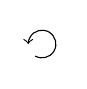
\begin{tikzpicture}[baseline]
    \draw[->](0, 0) arc (-120:180:.5em);
  \end{tikzpicture}
}

\begin{center}
  \begin{tikzcd}[column sep=tiny]
    \widetilde{X}\arrow[d] & \arrow[l, phantom, sloped, "\actson"] G \\ 
    \overline{X} \arrow[d] & \arrow[l, phantom, sloped, "\actson"] G/[K_G, K_G] \\ 
    X=S^3-K
  \end{tikzcd}
\end{center}

\begin{lemma}
  The following is a short exact sequence of chain complexes
  \begin{center}
    \begin{tikzcd}
      0 \arrow[r] & C_*(\overline{X})\arrow[r, "t-1"] & C_*(\overline{X})\arrow[r] & C_*(X)\arrow[r] & 0 
    \end{tikzcd}
  \end{center}
\end{lemma}
